%%%%%%%%%%%%%%%%%%%%%%%%%%%%%%%%%%%%%%%%%
% kaobook
% LaTeX Template
% Version 1.3 (18/2/20)
%
% This template originates from:
% https://www.LaTeXTemplates.com
%
% For the latest template development version and to make contributions:
% https://github.com/fmarotta/kaobook
%
% Authors:
% Federico Marotta (federicomarotta@mail.com)
% Giuseppe Silano (g.silano89@gmail.com)
% Based on the doctoral thesis of Ken Arroyo Ohori (https://3d.bk.tudelft.nl/ken/en)
% and on the Tufte-LaTeX class.
% Modified for LaTeX Templates by Vel (vel@latextemplates.com)
%
% License:
% CC0 1.0 Universal (see included MANIFEST.md file)
%
%%%%%%%%%%%%%%%%%%%%%%%%%%%%%%%%%%%%%%%%%

%----------------------------------------------------------------------------------------
%	PACKAGES AND OTHER DOCUMENT CONFIGURATIONS
%----------------------------------------------------------------------------------------

\documentclass[
	fontsize=10pt, % Base font size
	twoside=false, % Use different layouts for even and odd pages (in particular, if twoside=true, the margin column will be always on the outside)
	%open=any, % If twoside=true, uncomment this to force new chapters to start on any page, not only on right (odd) pages
	%chapterprefix=true, % Uncomment to use the word "Chapter" before chapter numbers everywhere they appear
	%chapterentrydots=true, % Uncomment to output dots from the chapter name to the page number in the table of contents
	numbers=noenddot, % Comment to output dots after chapter numbers; the most common values for this option are: enddot, noenddot and auto (see the KOMAScript documentation for an in-depth explanation)
	%draft=true, % If uncommented, rulers will be added in the header and footer
	%overfullrule=true, % If uncommented, overly long lines will be marked by a black box; useful for correcting spacing problems
]{kaobook}

% Choose the language
\usepackage[spanish, mexico]{babel} % traduce a español
\usepackage[autostyle]{csquotes} % comillas mexicanas
\usepackage{siunitx}
% Load packages for testing
%\usepackage{blindtext}
%\usepackage{showframe} % Uncomment to show boxes around the text area, margin, header and footer
%\usepackage{showlabels} % Uncomment to output the content of \label commands to the document where they are used

% Load the bibliography package
\usepackage{styles/kaobiblio}
\addbibresource{bib.bib} % Bibliography file
\usepackage[version=4]{mhchem}
\DeclareSIUnit\Molar{\textsc{m}}
% Load mathematical packages for theorems and related environments. NOTE: choose only one between 'mdftheorems' and 'plaintheorems'.
\usepackage{styles/mdftheorems}
\usepackage{subcaption}
%\usepackage{styles/plaintheorems}

\graphicspath{imgs/} % Paths in which to look for images

\makeindex[columns=3, title=Alphabetical Index, intoc] % Make LaTeX produce the files required to compile the index

\makeglossaries % Make LaTeX produce the files required to compile the glossary

\makenomenclature % Make LaTeX produce the files required to compile the nomenclature

%----------------------------------------------------------------------------------------

\begin{document}

%----------------------------------------------------------------------------------------
%	BOOK INFORMATION
%----------------------------------------------------------------------------------------

%\titlehead{Document Template}
% \subject{Subject}

\title[Efecto del pH en la condición de cristalización sobre el daño por radiación en cristales de proteína]{Efecto del pH en la condición de cristalización sobre el daño por radiación en cristales de proteína}
% \subtitle{Subtitle}

\author[FMP]{Francisco Murphy Pérez}

\date{\today}

%\publishers{An Awesome Publisher}

%----------------------------------------------------------------------------------------

\frontmatter % Denotes the start of the pre-document content, uses roman numerals

%----------------------------------------------------------------------------------------
%	OPENING PAGE
%----------------------------------------------------------------------------------------

% \makeatletter
% \extratitle{
% 	% In the title page, the title is vspaced by 9.5\baselineskip
% 	\vspace*{9\baselineskip}
% 	\vspace*{\parskip}
% 	\begin{center}
% 		% In the title page, \huge is set after the komafont for title
% 		\usekomafont{title}\huge\@title
% 	\end{center}
% }
% \makeatother

%----------------------------------------------------------------------------------------
%	COPYRIGHT PAGE
%----------------------------------------------------------------------------------------

\makeatletter
%\uppertitleback{\@titlehead} % Header

\lowertitleback{
%	\textbf{Disclaimer} \\
%	You can edit this page to suit your needs. For instance, here we have a no copyright statement, a colophon and some other information. This page is based on the corresponding page of Ken Arroyo Ohori's thesis, with minimal changes.
%	
	\medskip
%	
%	\textbf{No copyright} \\
%	\cczero\ This book is released into the public domain using the CC0 code. To the extent possible under law, I waive all copyright and related or neighbouring rights to this work.
%	
%	To view a copy of the CC0 code, visit: \\\url{http://creativecommons.org/publicdomain/zero/1.0/}
%	
	\medskip
	
	\textbf{Colofón} \\
Este documento se compuso con la ayuda de: \KOMAScript{} (\url{https://sourceforge.net/projects/koma-script/}) y \LaTeX{} (\url{https://www.latex-project.org/}), usando la plantilla denominada kaobook (\url{https://github.com/fmarotta/kaobook/}). 
	
	\medskip
	
	%\textbf{Publisher} \\
	%Primera versión mayo 2019%\@publishers
}
\makeatother

%----------------------------------------------------------------------------------------
%	DEDICATION
%----------------------------------------------------------------------------------------

\dedication{
A Lucía, por supuesto.	

}

%----------------------------------------------------------------------------------------
%	OUTPUT TITLE PAGE AND PREVIOUS
%----------------------------------------------------------------------------------------

% Note that \maketitle outputs the pages before here

% If twoside=false, \uppertitleback and \lowertitleback are not printed
% To overcome this issue, we set twoside=semi just before printing the title pages, and set it back to false just after the title pages
\KOMAoptions{twoside=semi}
\maketitle
\KOMAoptions{twoside=false}

%----------------------------------------------------------------------------------------
%	PREFACE
%----------------------------------------------------------------------------------------

\chapter*{Resumen}



%----------------------------------------------------------------------------------------
%	TABLE OF CONTENTS & LIST OF FIGURES/TABLES
%----------------------------------------------------------------------------------------

\begingroup % Local scope for the following commands

% Define the style for the TOC, LOF, and LOT
%\setstretch{1} % Uncomment to modify line spacing in the ToC
%\hypersetup{linkcolor=blue} % Uncomment to set the colour of links in the ToC
\setlength{\textheight}{23cm} % Manually adjust the height of the ToC pages

% Turn on compatibility mode for the etoc package
\etocstandarddisplaystyle % "toc display" as if etoc was not loaded
\etocstandardlines % "toc lines as if etoc was not loaded

\tableofcontents % Output the table of contents

\listoffigures % Output the list of figures

% Comment both of the following lines to have the LOF and the LOT on different pages
%\let\cleardoublepage\bigskip
%\let\clearpage\bigskip

\listoftables % Output the list of tables


\newacronym{api}{API}{Application Programming Interface }
\newacronym{pdb}{PDB}{Protein Data Bank}
\newacronym{crx}{CRX}{Cristalografía de rayos X}
\newacronym{ccd}{CCD}{Charge-coupled device}
\newacronym{xfel}{XFEL}{X-ray Free Electron Laser}
\newacronym{iupac}{IUPAC}{International Union of Pure and Applied Chemistry}
\setglossarystyle{listgroup} % Set the style of the glossary (see https://en.wikibooks.org/wiki/LaTeX/Glossary for a reference)
\printglossary[title=Acrónimos, toctitle=Acrónimos] % Output the glossary, 'title' is the chapter heading for the glossary, toctitle is the table of contents heading

\endgroup

%----------------------------------------------------------------------------------------
%	MAIN BODY
%----------------------------------------------------------------------------------------

\mainmatter % Denotes the start of the main document content, resets page numbering and uses arabic numbers
\setchapterstyle{kao} % Choose the default chapter heading style

\chapter{Introducción}
\section{Cristalografía de rayos X}
Actualmente la forma preponderante de obtener la estructura atómica de una macromolécula es a través de la cristalografía de rayos X (tabla \ref{tab:pdb-stats}). 

\begin{table}[h]
	\centering
	\begin{tabular}{@{}llr@{}}
		\toprule
		Método experimental & Total  & Porcentaje        \\ \midrule
		CRX     & 146963 & 88.84	\\
		RMN     & 13005  & 7.86		\\
		CME     & 5181   & 3.13		\\
		Varios  & 167    & 0.10		\\
		Otros 	& 106    & 0.06		\\
		Total   & 165422 & 100		\\ \bottomrule
	\end{tabular}%
	\caption[Número de estructuras depositadas por método experimental]{Número de estructuras depositadas en el PDB por método experimental. TODO: Falta explicar qué significa cada cosa.}
	\label{tab:pdb-stats}
\end{table}

De manera muy somera, el experimento de cristalografía de rayos X consiste en:

\begin{enumerate}
	\item Incidir rayos X sobre el cristal de la macromolécula de interés. 
	\item Obtener el patrón de difracción. 
	\item Rotar el cristal en cierto eje. 
	\item Repetir los pasos anteriores $n$ veces.
\end{enumerate}

Dos puntos que cabe resaltar son los siguientes: (\emph{i}) Los rayos X son difractados dentro del cristal macromolecular y dada la estructura repetitiva del mismo, se puede obtener una amplificación de este proceso puramente físico. Los rayos X difractados contienen información de la estructura macromolecular, por lo que es necesario detectarlos y mantener una copia digital de cada patrón de difracción para su posterior análisis. (\emph{ii}) En general, existen reglas de dedo para obtener un estimado útil de $n$ TODO: cita. 

Entre mayor información se obtenga, los pasos subsecuentes se vuelven menos complicados, por lo que sería fácil asumir que uno necesita exponer el cristal macromolecular cientos o miles de veces al haz de rayos X. Sin embargo, esto es raramente posible. El problema consiste en que los rayos X tienen la energía suficiente para ionizar la materia. En el caso de un cristal macromolecular, su estabilidad física se da por interacciones no covalentes, por lo que su desintegración no requiere de mucha energía. Además es evidente que al perderse el orden cristalino se pierde la amplificación del proceso de difracción y en consecuencia los patrones de difracción cada vez contienen menos información. Esto se conoce como daño por radiación y es una de las grandes limitantes de la cristalografía de rayos X.


\section{Crioprotección y desarrollo tecnológico de sincrotrones}

La primer estructura macromolecular determinada fue aquella de la mioglobina en 1958 \cite{Kendrew1958}. La forma de contender con el daño por radiación en aquellas épocas era utilizando decenas de cristales y promediar los patrones de difracción. Para 1966 es evidente que enfriar el cristal durante su exposición a los rayos X, ayuda a disminuir el daño por radiación \cite{Low1966}. La criocristalografía se desarrolla en los años siguientes y es hasta el año 2000 que se utiliza de manera rutinaria \cite{Garman2003}. Para entonces la noción general en el campo de la criocristalografía es que el daño por radiación era insignificante. Precisamente esta noción cambia en el mismo año, cuando tres estudios independientes muestran el efecto del daño por radiación en la entonces nueva generación de sincrotrones \cite{Teng2000, Ravelli2000, Weik2000}.

Una de las principales fuentes de rayos X es la radiación de sincrotrón. Una de las características de un sincrotrón es su brillo espectral\sidenote{Se define como la distribución del flujo de fotones en el espacio y el rango angular. El flujo se establece a su vez como el número de fotones por segundo que atraviesan un área definida por un ancho de banda dado \cite{Willmott2019}.}. La revolución tecnológica de los sincrotrones se nota en la diferencia del orden de magnitud del brillo espectral. Este aumento se ha permitido a pesar de que existe un incremento en el daño por radiación, porque da acceso a una gran ventaja: la posibilidad de utilizar cristales de menor tamaño\sidenote{La principal limitante de la cristalografía es obtener cristales macromoleculares de un tamaño adecuado: para una línea común esto significa al menos cien micrómetros en sus tres dimensiones, para una línea microfoco este valor puede disminuir un orden de magnitud.}.  Actualmente se está desarrollando la tecnología para cambiar la metodología de la colecta de datos, usando cristales macromoleculares nanométricos y con una fuente de rayos X más poderosa denominada XFEL (del inglés \emph{X-ray Free Electron Laser}) \cite{Martin-Garcia2016}. Existen ya varios estudios en los que se ha demostrado la posibilidad de obtener estructuras macromoleculares con esta nueva metodología \cite{Martin-Garcia2016}. Sin embargo, el acceso al tiempo experimental en un XFEL es actualmente muy limitado.

\section{Radioprotectores}
Al ser evidente que el daño por radiación aumentaba con el incremento en brillo, fue necesario buscar alternativas que ayudaran a mitigar el daño por radiación. Se han investigado alternativas pre y posteriores a la difracción con varios enfoques en los últimos 20 años\cite{Garman2017}. Una de las alternativas que resalta es el uso de moléculas pequeñas que interactuan con los radicales libres generados por la radiación. Estas moléculas se denominan radioprotectores.  Sin embargo, en la literatura científica existen varias incongruencias con respecto a la efectividad de los radioprotectores y es por esto que la comunidad cristalográfica no ha adoptado al cien por ciento el uso de radioprotectores de manera rutinaria \cite{Nowak2009, Allan2013}.

\chapter{Antecedentes}
\labch{antec}
\section{pH}
\labsec{ph}
Una estrategia innovadora, investigada en la tesis de maestría del presente autor%\sidenote{Disponible en el siguiente enlace \url{https://github.com/murpholinox/tesis\_maestria}}
, fue modificar el pH dentro de los cristales macromoleculares. Esta idea se basa en la idea general de los radioprotectores y se detalla a continuación. 

La radiólisis del agua produce las siguientes reacciones \sidecite{VonSonntag2006}:
\begin{align}
	\ce{H2O           &->[rayos X]     H2O^{.+}    +             e^{-}}  \\
	\ce{H2O           &->[rayos X]     H2O^{*}}                          \\
	\ce{H2O^{.+}      &->  \color{red}HO^{.}       +              H^{+}} \\
	\ce{e^{-} + nH2O  &->  \color{red}e^{-}_{solv.}}                     \\
	\ce{H2O^{*}       &->  \color{red}HO^{.}       +   \color{red}H^{.}}
\end{align} 
Donde las especies químicas denotadas en rojo, representan los primeros radicales libres presentes en un cristal macromolecular (el radical hidroxilo, el electrón solvatado y el radical hidrógeno).% Esto es relevante porque en general el contenido de solvente, agua, en un cristal macromolecular es bastante. 

Con la criocristalografía de rayos X, se impide la difusión del radical hidroxilo \sidecite{Owen2012a}. Sin embargo, el \ce{e^{-}_{solv.}} y el radical hidrógeno todavía son móviles. El electrón solvatado puede moverse del solvente a la proteína, donde es capaz de viajar a través de la cadena polipeptídica hasta hallar un centro electrofílico, como por ejemplo átomos metálicos o puentes disulfuro (véase la \reffig{fig:symons92}) \sidecite{Symons1997}. Esta es la razón del origen del orden en el que se presenta el daño por radiación específico, pues la captura de electrones es mucho más específica que la captura de huecos positivos \sidecite{Close2019}. Por su parte, el radical hidrógeno sigue una reacción de recombinación formando como producto final \ce{H2}, al parecer el responsable directo del daño por radiación global \sidecite{Meents2010}.

\begin{figure}[h]
	\centering
	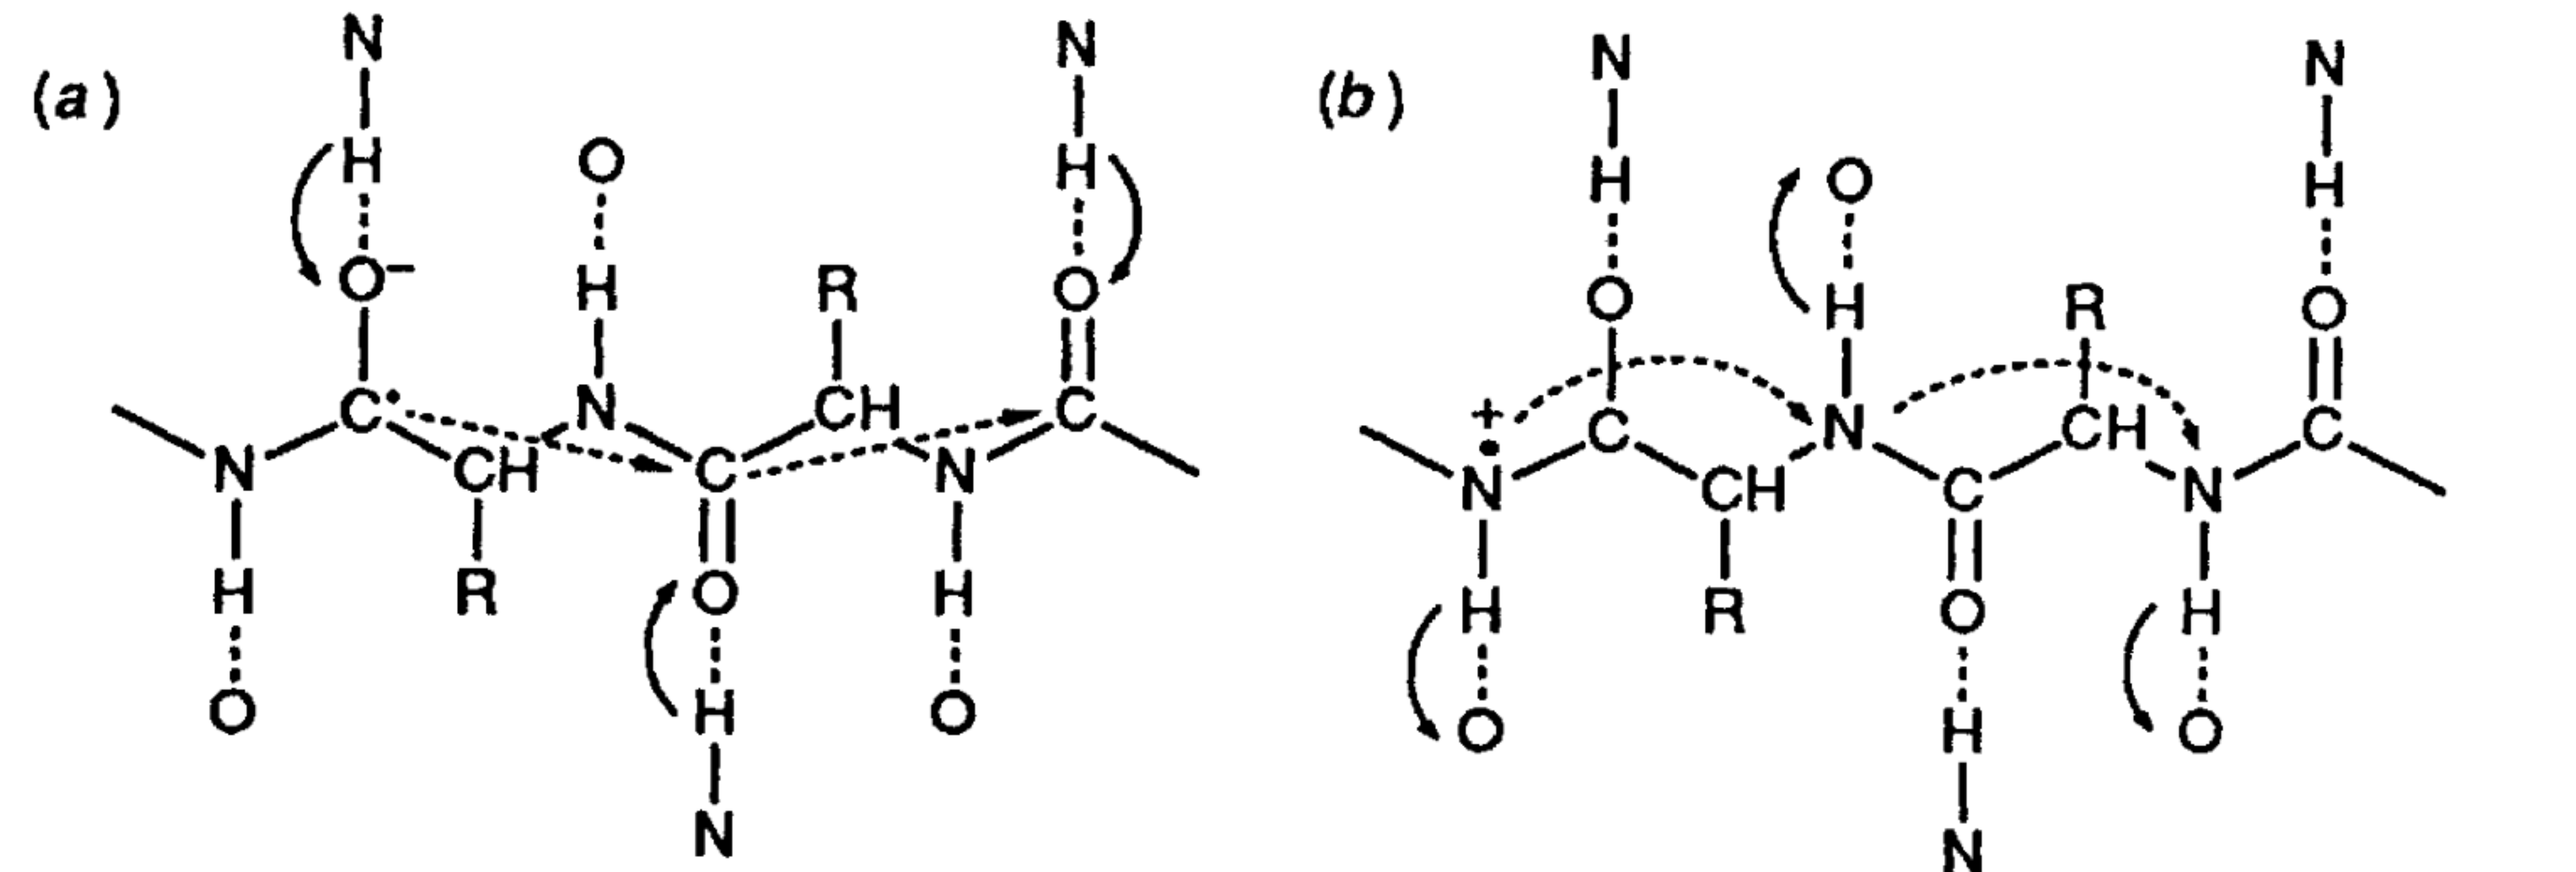
\includegraphics[width=0.9\textwidth]{imgs/symons92.png}
	\caption[Movimiento de cargas en la cadena polipeptídica]{Moviento de electrones (a) y huecos positivos (b), a través de la cadena polipeptídica. Fuente: \cite{Symons1997}.}
	\labfig{fig:symons92}
\end{figure}

El electrón solvatado y el átomo de hidrógeno se encuentran en un equilibrio ácido-base; por lo que el electrón solvatado se convierte en \ce{H^{.}} en una solución ácida. %De hecho, en el campo de la química de las radiaciones, es común estudiar el efecto de un radical al convertir los otros radicales en especies el radical estudiado. 
\begin{equation}
\ce{e^{-}_{solv.} + H^{+} <=> H^{.}}
\end{equation}

En la tesis de maestría se usó como sistema de estudio la lisozima de clara de huevo de gallina, que presenta cuatro puentes disulfuro. La idea era que el ion hidronio, también conocido como oxidanio, funcionara como radioprotector al interactuar con los electrones solvatados antes que estos interactuaran con los puentes disulfuro de esta proteína. Para esto, se comparó el daño específico sobre los puentes disulfuro en cristales de lisozima a tres niveles de p: \num{3.7}, \num{4.7} y \num{5.7}. Los resultados obtenidos fueron opuestos a los esperados: a niveles comparables de dosis de radiación absorbida, el cristal con el pH más ácido presentó mayor daño por radiación que el cristal con el pH más básico.

La variabilidad entre cristales macromoleculares, aún proveniendo de la misma condición de cristalización, puede llevar a conclusiones erróneas \sidecite{Nowak2009}. En la tesis de maestría no se pudo concluir si la diferencia observada era estadísticamente significativa, pues no se realizaron las repeticiones necesarias para cada condición experimental.



\chapter{Objetivo}
\labch{objet}

El objetivo de este proyecto es determinar el efecto del pH en la condición de cristalización de ciertas proteínas sobre el daño por radiación. 
\section{Objetivos particulares}
\labsec{objpar}
Para lograr el objetivo principal de este proyecto, se plantean los siguientes objetivos particulares:

\begin{enumerate}
	\item Hallar una lista de proteínas capaces de cristalizar en un intervalo de pH \emph{amplio}.
	\item Cristalizar las proteínas, cada una en la misma condición, pero a diferentes pHs.
	\item Difractarlas.
	\item Obtener las estructuras.
	\item Realizar un análisis del daño por radiación específico con mapas de diferencia de densidad electrónica.
\end{enumerate}	
\chapter{Materiales y métodos}
\labch{mayme}

El \acrshort{pdb} contiene información acerca de cientos de miles de proteínas cristalizadas en diferentes condiciones de cristalización. Para hallar qué proteínas pueden cristalizar en un amplio intervalo de pH se realizó un análisis \emph{in silico}, como se explica brevemente\sidenote{Con detalle en \url{https://github.com/murpholinox/doctorado}.} a continuación. 

\subsection{Extracción de datos}
%\sidenote{Actualmente la API fue reemplazada por una nueva versión cuyo desarrollo no ha sido completado \url{https://tinyurl.com/y84kuvs7}.}
Se decidió emplear la información cruda del \acrshort{pdb}, es decir, extraer la información experimental necesaria directamente del cabezal de los archivos de las estructuras depositadas en el \acrshort{pdb}. La principal ventaja es que la extracción de información es de una manera más directa, sin depender de la interfaz de programación de aplicaciones (\acrshort{api}, por sus siglas en inglés) del mismo \acrshort{pdb}. Para extraer la información de los cabezales se usó el programa \Package{gemmi}\sidenote{Disponible en el siguiente enlace \url{https://github.com/project-gemmi/gemmi}.}. La información extraída es la siguiente: el contador de la entidad macromolecular, el tipo de entidad, el código de acceso de la base de datos de referencia\sidenote{La mayoría de las veces el código usado es aquél de la base de datos UniProt \url{https://www.uniprot.org/}.}, su descripción, el método experimental para crecer los cristales, el pH de la condición de cristalización, los detalles del experimento de la cristalización, la resolución final del modelo estructural, el grupo espacial en el que cristaliza la macromolécula y el identificador de objeto digital de la publicación científica correspondiente. A continuación se muestra un ejemplo de la información extraída:

\begin{kaobox}[frametitle=Ejemplo 1]
\begin{verbatim}
6LU7,1,polypeptide(L),P0DTD1,main protease,EVAPORATION,\
6,"2% polyethylene glycol (PEG) 6000, 3% DMSO, 1mM DTT,\
0.1M MES buffer (pH 6.0), protein concentration 5mg/ml,\
VAPOR DIFFUSION, HANGING DROP, temperature 293K",2.16,\
2.16,C 1 2 1,10.1038/s41586-020-2223-y,21728,210031
6LU7,2,polypeptide(L),P0DTD1,main protease,EVAPORATION,\
6,"2% polyethylene glycol (PEG) 6000, 3% DMSO, 1mM DTT,\
0.1M MES buffer (pH 6.0), protein concentration 5mg/ml,\
VAPOR DIFFUSION, HANGING DROP, temperature 293K",2.16,\
2.16,C 1 2 1,10.1038/s41586-020-2223-y,21728,210031
\end{verbatim}
\end{kaobox}

El resultado final es una tabla de datos, con \num{226523} observaciones, o filas, y \num{14} variables, o columnas. El número de observaciones es mayor que el número de estructuras en el \acrshort{pdb}, esto es debido a que cada archivo puede tener más de una macromolécula\sidenote{Como es el caso del ejemplo 1.}. %La integridad de los datos se demuestra con una gráfica.

\subsection{Limpieza de datos}
Se aplican los siguientes filtros a los datos extraídos para eliminar observaciones que:

\begin{enumerate}
	\item Carecen de código de acceso.
	\item Tienen una resolución peor que \SI{2}{\angstrom}. 
	\item Carecen del valor de pH de la condición de cristalización.
	\item El número de entidades es mayor o igual a dos.
\end{enumerate}

La lógica de los filtros es la siguiente: (\num{1} y \num{3}) Remover entradas que no tengan las anotaciones correspondientes\sidenote{Desafortunadamente la información experimental no siempre se encuentra disponible en los archivos del PDB.}, en este caso el código de acceso de la proteína y el pH de la condición de cristalización. La última es la anotación más relevante para este proyecto y la primera es la única manera de conocer casi inequívocamente la proteína representada en el archivo. (\num{2}) La resolución final del modelo estructural es un indicador de la calidad del cristal obtenido, a mayor resolución menos defectos posee el cristal. Este filtro garantizará que el listado de proteínas obtenidas sean fáciles de cristalizar. Además este filtro servirá para el análisis posterior, al comparar el daño por radiación específico, pues los resultados serán más confiables con una buena resolución. (\num{4}) Como se mencionó anteriormente, un archivo puede contener múltiples macromoléculas. Este filtro ayuda a descartar proteínas cristalizadas con otras. En general, las condiciones de cristalización para combinaciones diferentes de macromoléculas serán diferentes, por lo que no tiene caso tener varias observaciones de la misma proteína si presenta diferentes compañeros. 

En la tabla \reftab{tab:top50}, se muestran las 50 proteínas más representadas en los datos que cumplen los primeros cuatros filtros. A partir de las cuales se aplican los siguientes dos filtros, que ayudan a eliminar las observaciones donde:

\begin{enumerate}
	\setcounter{enumi}{4}
	\item Su secuencia de aminoácidos sea diferente de la secuencia consenso para cada conjunto de proteínas.
	\item No presenten un intervalo de pH amplio en su cristalización.
\end{enumerate}

La lógica de estos dos filtros es la siguiente: (\num{5}) en el primer filtro se alegó que el código de acceso de UniProt es la manera de conocer \emph{casi inequívocamente la proteína representada}. En el caso de algunos virus, el código corresponde a un gen que puede codificar para diferentes proteínas. Debido a esto se realizó un alineamiento múltiple, con el programa \Package{mafft} \sidecite{Katoh2013},  para eliminar proteínas distintas a la respectiva secuencia consenso con el mismo código de acceso. A continuación se muestra un ejemplo:

\begin{kaobox}[frametitle=Ejemplo 2]
	\begin{verbatim}
	6W4H,1,polypeptide(L),P0DTD1,SARS-CoV-2 NSP16,...
	6W4H,2,polypeptide(L),P0DTD1,SARS-CoV-2 NSP16,...
	6W6Y,1,polypeptide(L),P0DTD1,SARS-CoV-2 NSP3,...
	6WQD,1,polypeptide(L),P0DTD1,SARS-CoV-2 NSP7,...
	6WQD,2,polypeptide(L),P0DTD1,SARS-CoV-2 NSP7,...
	7BUY,1,polypeptide(L),7BUY,SARS-CoV-2 virus Main protease,
	\end{verbatim}
\end{kaobox}

Es claro que el código, \texttt{P0DTD1}, es el mismo; sin embargo, las observaciones corresponden a diferentes proteínas. Este filtro ayuda a mantener proteínas en las que su secuencia no difiera entre sí por más de 15 aminoácidos. Se mantienen entonces proteínas que difieran entre sí por la etiqueta de polihistidinas, pero se excluyen proteínas que contengan el péptido señal y proteínas quimeras, por ejemplo. Y (\num{6}) es la condición experimental que nos interesa en este proyecto, proteínas que cristalicen en un amplio intervalo de pH. Este filtro se aplicó por partes. Primero se realizó un gráfico de caja para cada una de las 50 proteínas más representadas en los datos. Este tipo de gráfica da una representación visual de la distribución de la variable en cuestión. Si la distribución no cubre al menos tres unidades de pH, entonces se descarta dicha proteína, en caso contrario se mantiene. De las proteínas restantes, 25, se realiza un histograma de frecuencias para determinar de manera cuantitativa la frecuencia con la que cada proteína ha sido cristalizada en valores de pH diferentes. Si la frecuencia no es mayor a cinco para la mayoría de las barras en cada histograma, la proteína se descarta, si no se mantiene (véase la \reffig{fig:vis-anal}). Esto resulta en un listado de 14 proteínas, donde las diez primeras entradas se presentan a continuación (véase la \reftab{tab:list}). 

\begin{table}[h]
	\centering
	\begin{tabular}{@{}llll@{}}
		\toprule
		Número & Código & Intervalo       & Nombre                              \\ \midrule
		1      & P00918 & 6               & Anhidrasa carbónica                 \\
		2      & P00698 & 5.5             & Lisozima                            \\
		3      & P00760 & 6               & Tripsina                            \\
		4      & P02766 & 5               & Transtiretina                       \\
		5      & P42212 & 6               & Proteína verde fluorescente         \\
		6      & O60885 & 3.5             & Proteína bromodominio 4             \\
		7      & P19491 & 4.5             & Receptor de glutamato 2             \\
		8      & O26232 & 4               & Orotidina-5’-fosfato descarboxilasa \\
		9      & P00772 & 4.5             & Elastasa                            \\
		10     & P00644 & 3               & Termonucleasa                       \\
\bottomrule
	\end{tabular}
	\caption[Proteínas que cristalizan en un intervalo amplio de pH]{Proteínas que cristalizan en un intervalo amplio de pH.}
	\labtab{tab:list}
\end{table}

\section{Colecta y análisis de datos}
Los cristales obtenidos serán difractados en un sincrotrón, midiendo la dosis de radiación absorbida. Para cada proteína se tendrán que realizar colectas de datos secuenciales de manera repetitiva. Gracias a la presencia de modelos estructurales en el \acrshort{pdb}, se puede estimar la dosis absorbida por la proteína antes de realizar el experimento de difracción. Esto se puede realizar gracias al programa \Package{raddose} \sidecite{Zeldin2013}. Se resolveran las estructuras por reemplazo molecular y se crearán mapas de diferencia de densidad electrónica para analizar la diferencia en daño por radiación específico a distintos pHs al mismo nivel de dosis de radiación absorbida. %Cabe señalar que la mayor parte del análisis posterior a la colecta de datos será \emph{in silico} y gracias al trabajo anterior se dispone de un flujo de trabajo semiautomático lo que facilitará en gran medida el presente proyecto.


%\pagelayout{wide} % No margins
%\addpart{Title of the Part}
%\pagelayout{margin} % Restore margins

%\chapter{Second Chapter}

\appendix % From here onwards, chapters are numbered with letters, as is the appendix convention

%\pagelayout{wide} % No margins
%\addpart{Appendix}
%\pagelayout{wide} % Restore margins
\chapter{Proteínas más representadas}
\labch{top50}

\begin{table}[h]
	\centering
	\begin{tabular}{@{}llllll@{}}
	\toprule
	Número & Código    & Cuenta & No. & Código       & Cuenta \\* \midrule

1      & \texttt{P11838} & 689    & 26     & \texttt{P23497}     & 106  \\
2      & \texttt{P00918} & 619    & 27     & \texttt{P00800}     & 103  \\
3      & \texttt{P00698} & 498    & 28     & \texttt{O26232}     & 102  \\
4      & \texttt{P00760} & 310    & 29     & \texttt{P22629}     & 97   \\
5      & \texttt{Q6PJP8} & 296    & 30     & \texttt{P00489}     & 96   \\
6      & \texttt{Q6B0I6} & 269    & 31     & \texttt{P03367}     & 96   \\
7      & \texttt{P02766} & 258    & 32     & \texttt{P68400}     & 95   \\
8      & \texttt{O95696} & 257    & 33     & \texttt{A0A073FPA6} & 84   \\
9      & \texttt{Q9UIF8} & 227    & 34     & \texttt{P46881}     & 79   \\
10     & \texttt{P00644} & 216    & 35     & \texttt{P00811}     & 78   \\
11     & \texttt{P00720} & 215    & 36     & \texttt{Q16539}     & 77   \\
12     & \texttt{P24941} & 203    & 37     & \texttt{P14174}     & 75   \\
13     & \texttt{P42212} & 182    & 38     & \texttt{P00431}     & 73   \\
14     & \texttt{P29476} & 178    & 39     & \texttt{P01116}     & 73   \\
15     & \texttt{P02185} & 172    & 40     & \texttt{P00183}     & 72   \\
16     & \texttt{O60885} & 170    & 41     & \texttt{P01112}     & 72   \\
17     & \texttt{P18031} & 152    & 42     & \texttt{Q00511}     & 70   \\
18     & \texttt{P61823} & 145    & 43     & \texttt{Q76353}     & 68   \\
19     & \texttt{P28720} & 144    & 44     & \texttt{P00282}     & 64   \\
20     & \texttt{P07900} & 142    & 45     & \texttt{P02883}     & 63   \\
21     & \texttt{P61626} & 139    & 46     & \texttt{P02945}     & 63   \\
22     & \texttt{P15121} & 125    & 47     & \texttt{P06873}     & 63   \\
23     & \texttt{P56817} & 124    & 48     & \texttt{P16113}     & 63   \\
24     & \texttt{P0DTD1} & 123    & 49     & \texttt{Q04609}     & 63   \\
25     & \texttt{P19491} & 116    & 50     & \texttt{P00772}     & 61   \\ \bottomrule
	\caption[Las 50 proteínas más representadas]{Las 50 proteínas más representadas en los datos, después de los cuatro primeros filtros. Eliminando estructuras que no contienen: código de acceso ni el valor de pH de la condición experimental. Además descarta aquellas estructuras con una resolución peor que \SI{2}{\angstrom} y donde el número de entidades es mayor o igual a dos.}
	\labtab{tab:top50}
	\end{tabular}
\end{table}


\chapter{Análisis visual}
\labch{vis-anal}
\begin{figure}[h!]
	\centering
	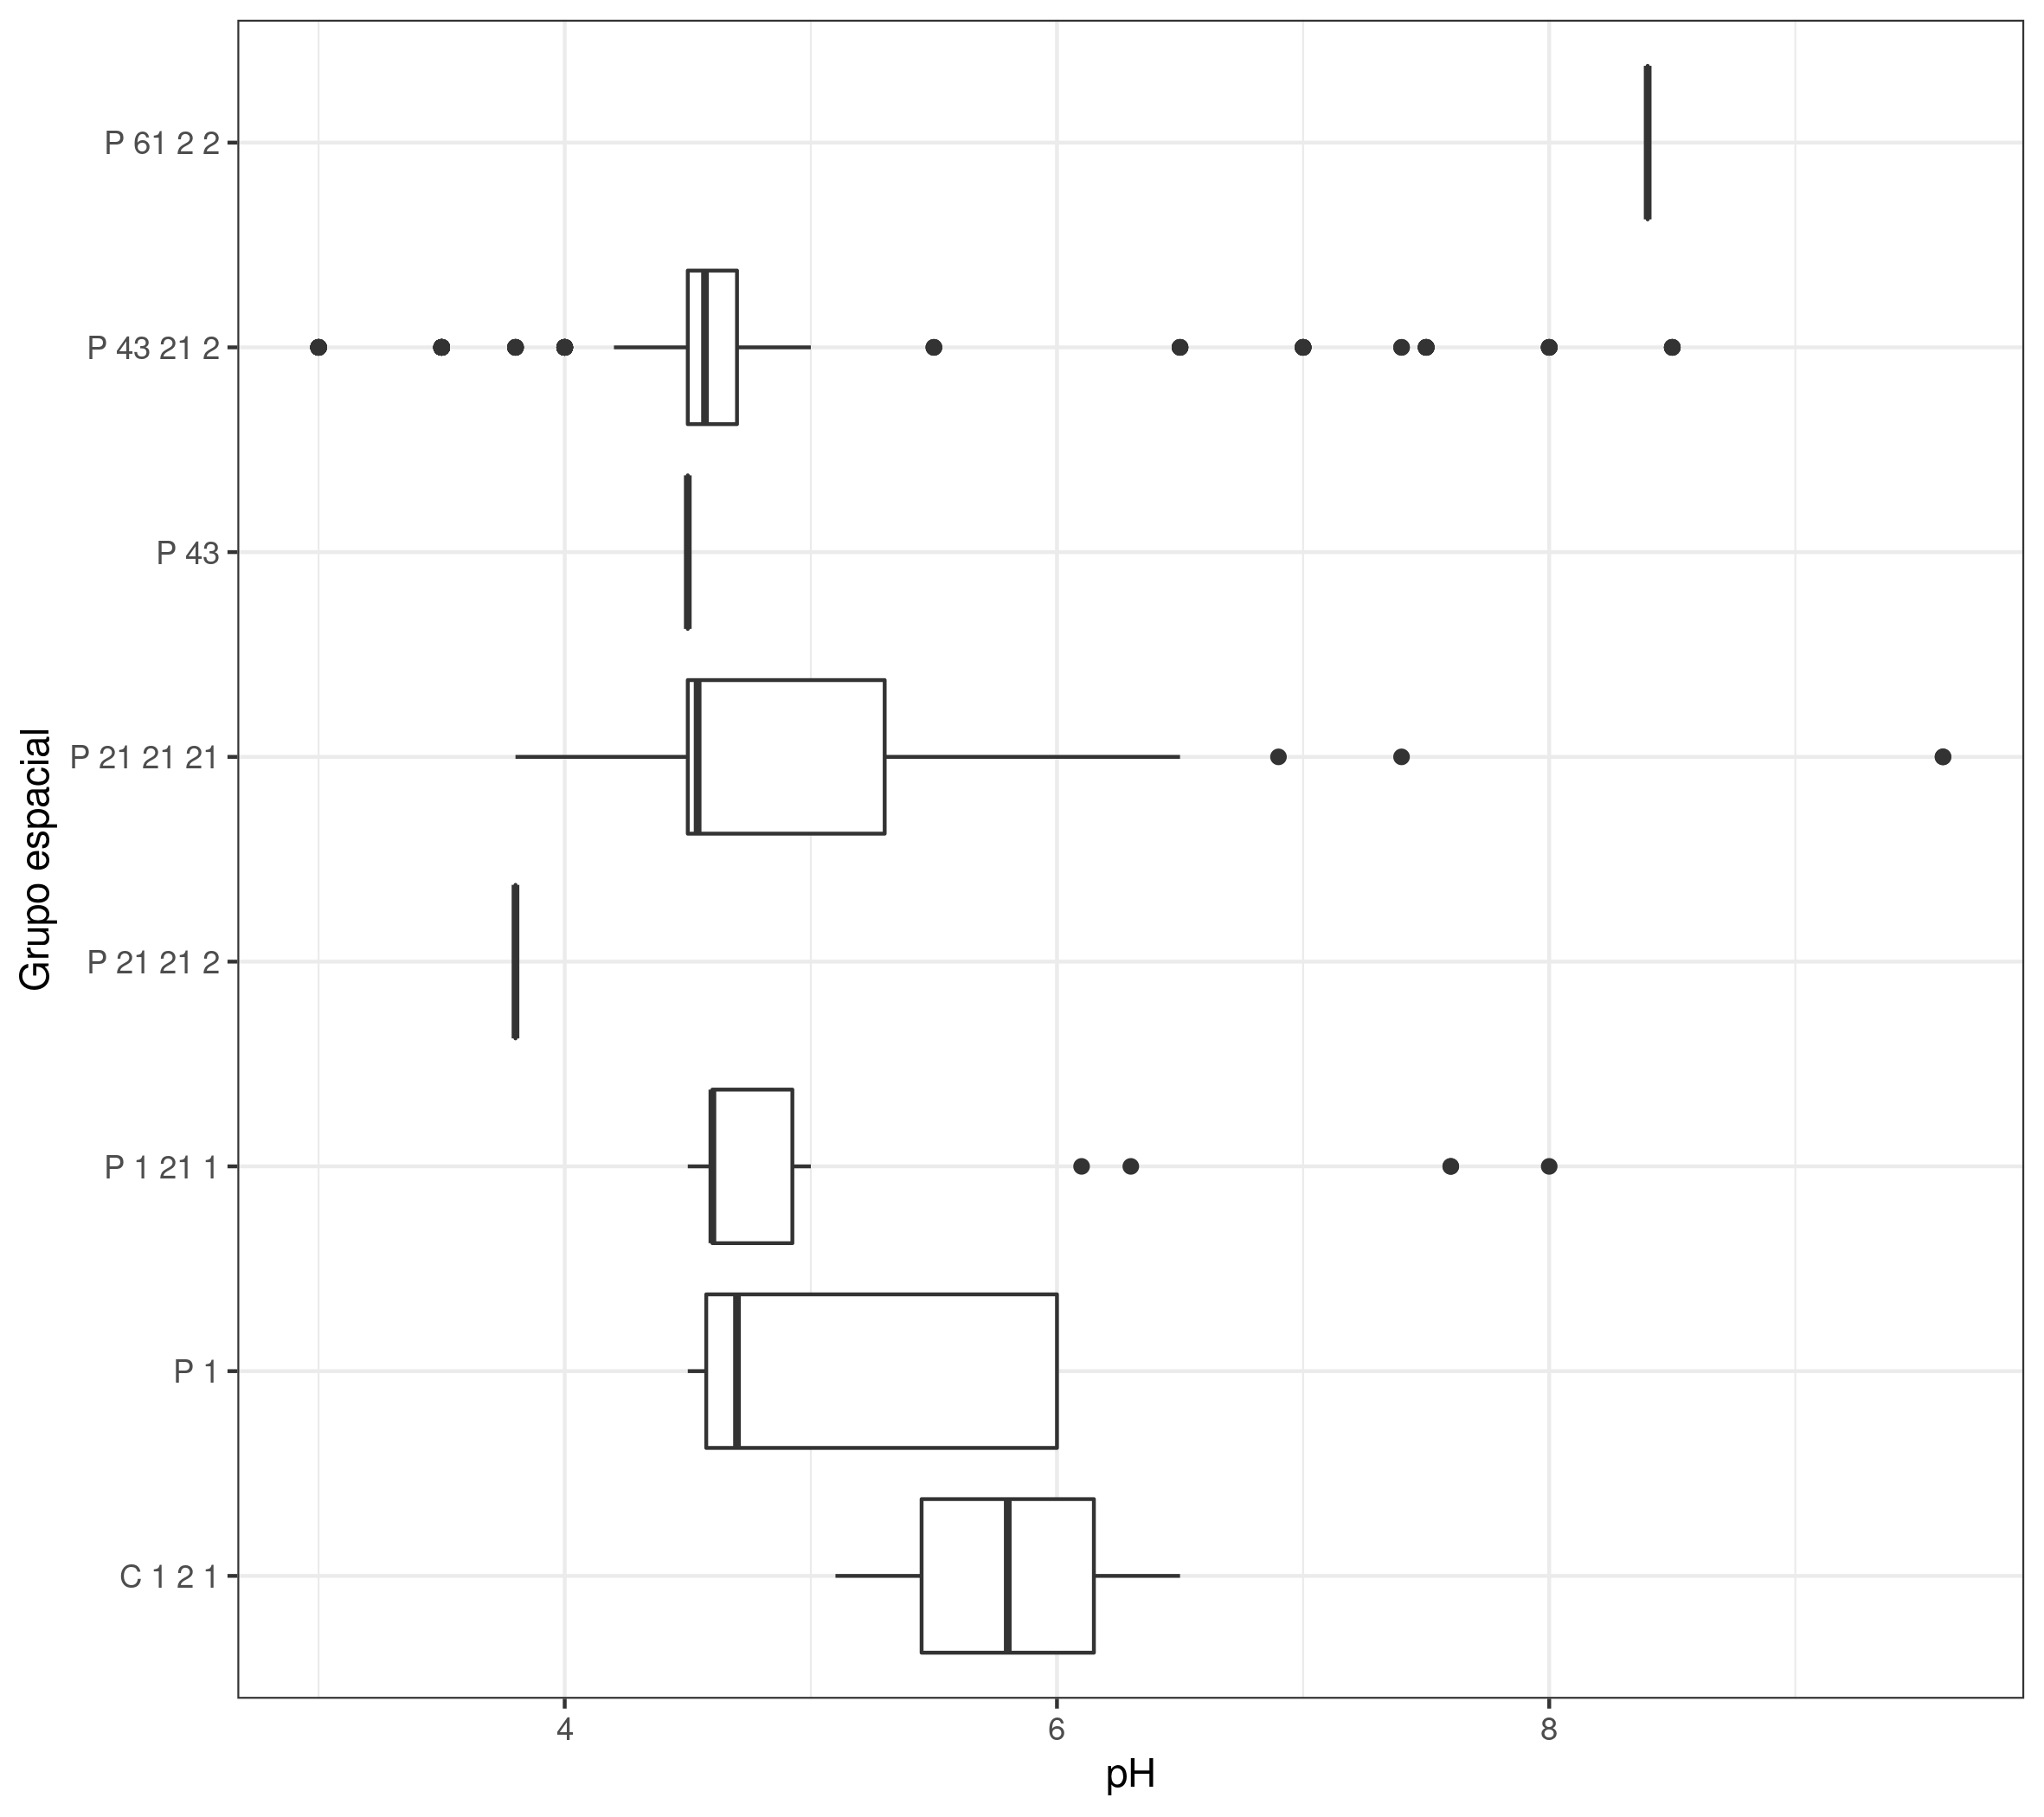
\includegraphics[width=0.8\textwidth]{imgs/box_pH_by_gpo_P00698}
	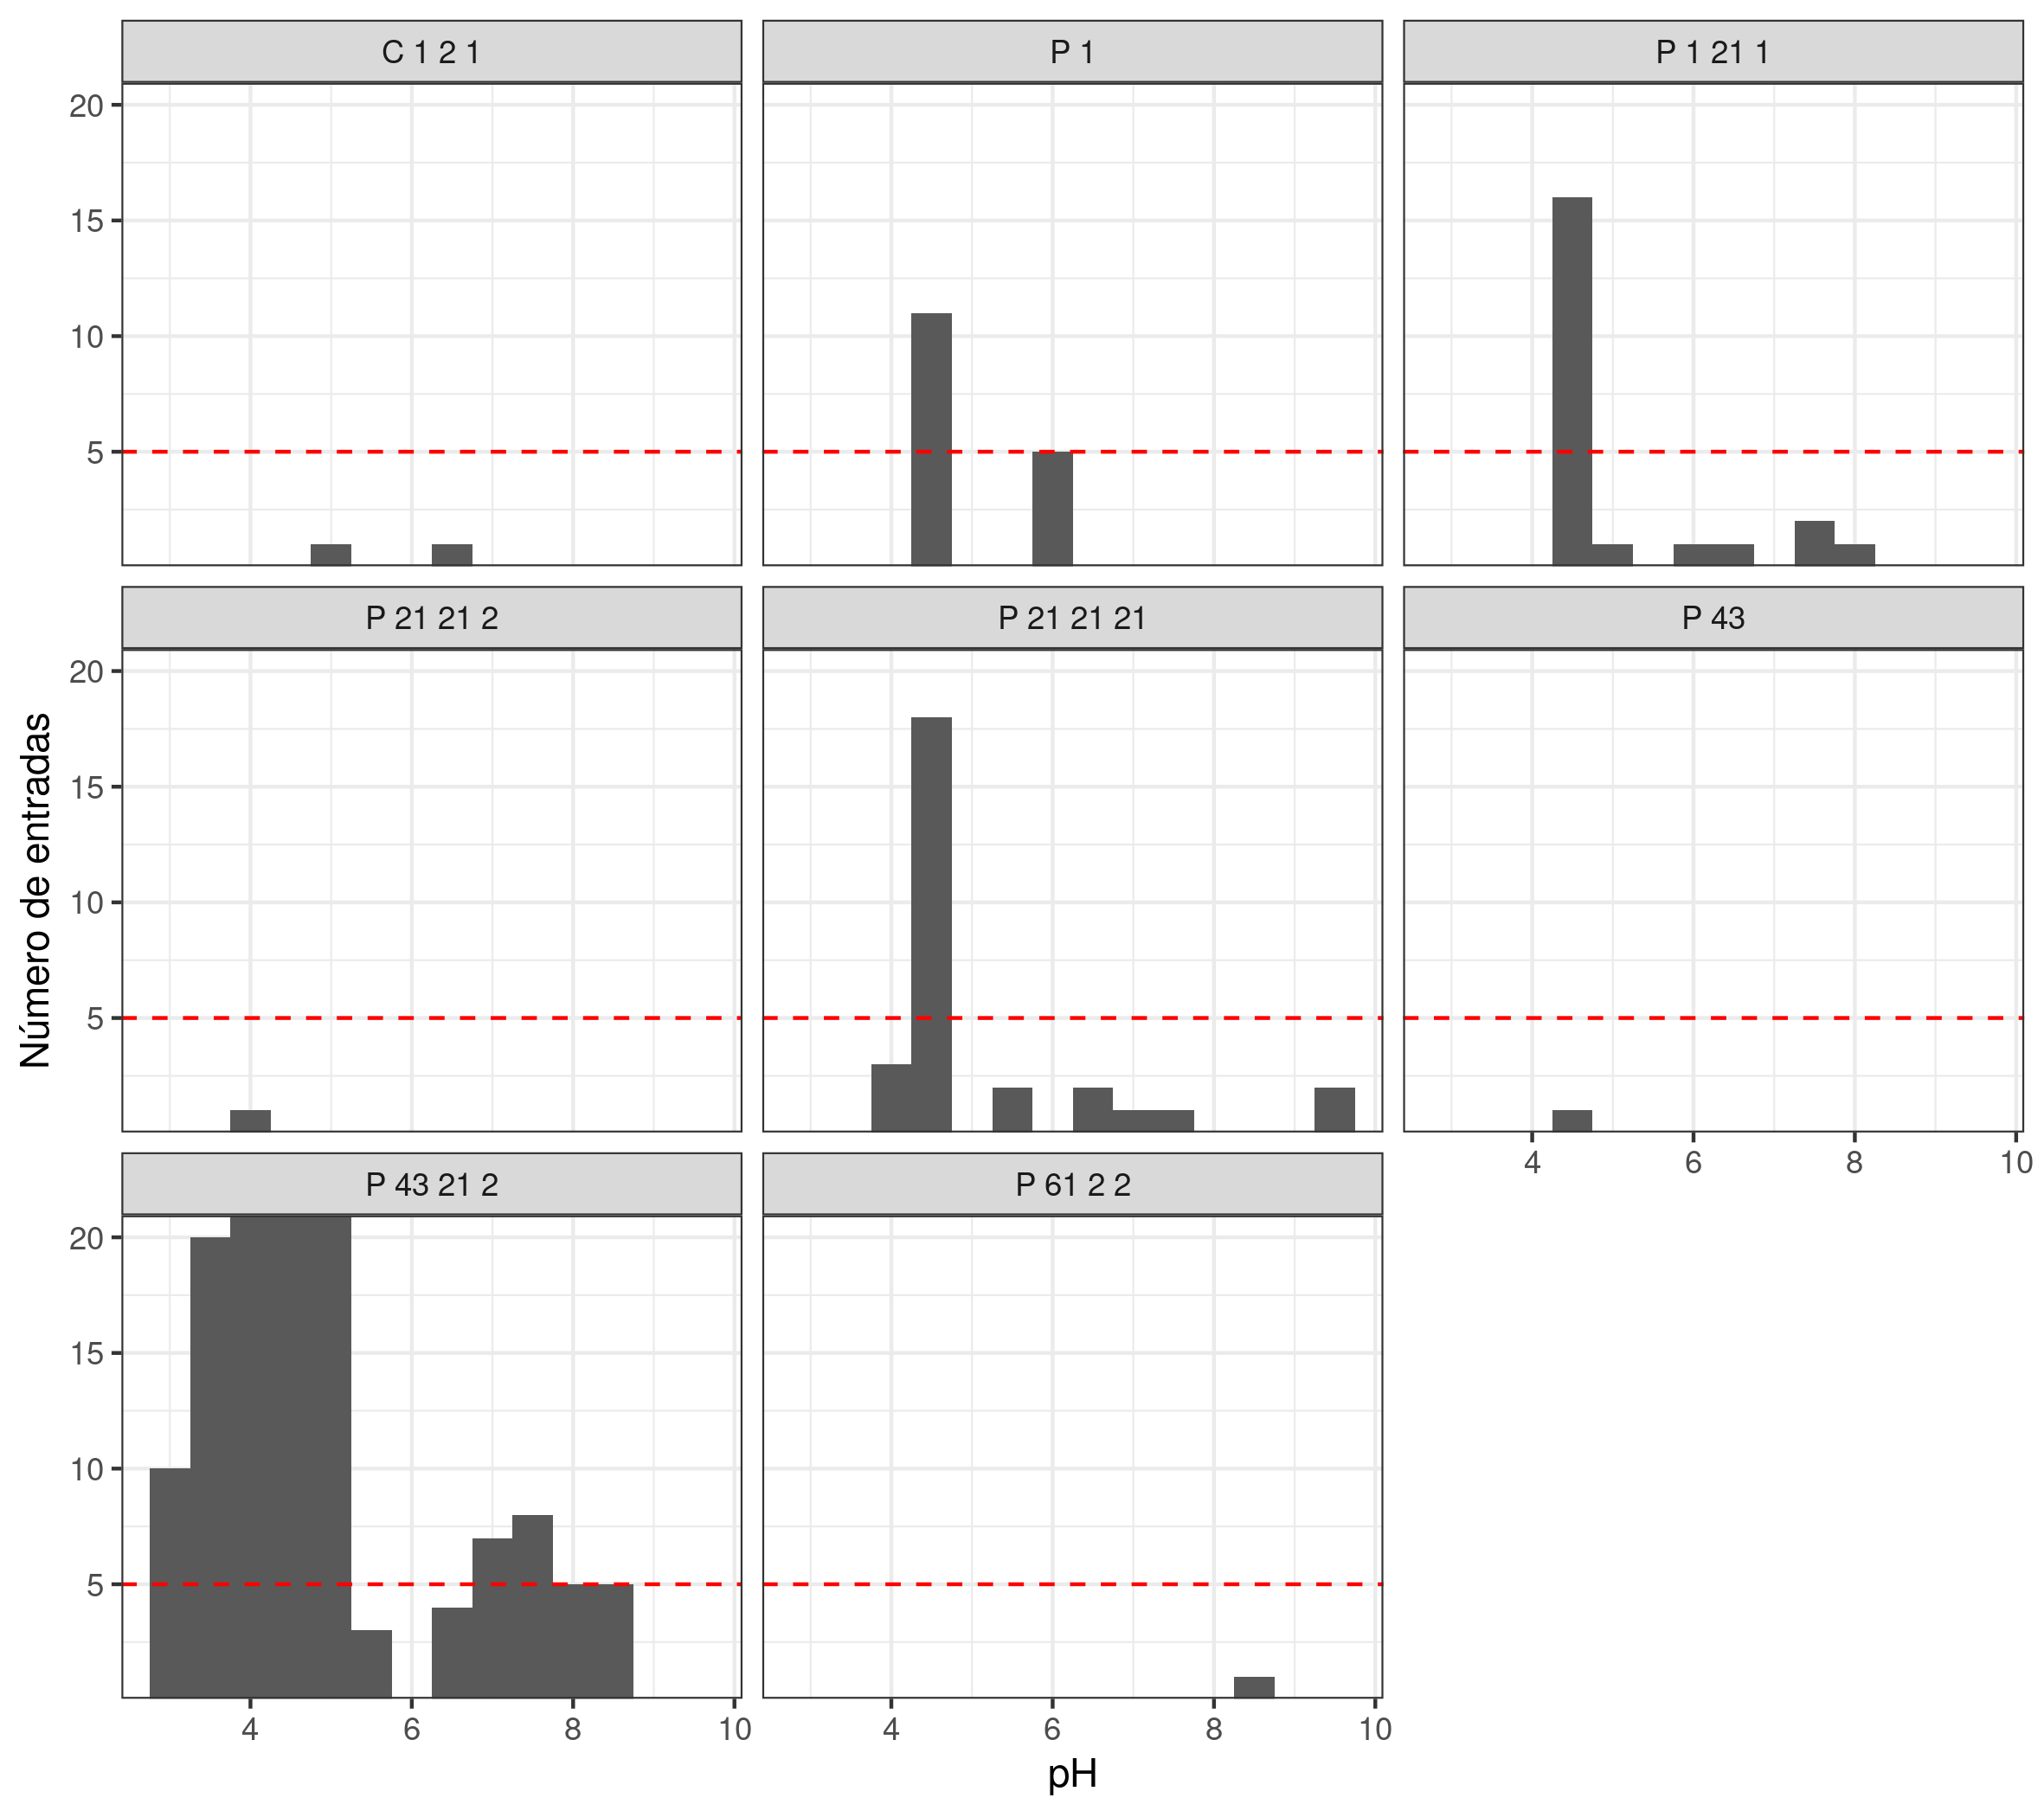
\includegraphics[width=0.8\textwidth]{imgs/hist_pH_by_gpo_P00698}
	\caption[Análisis visual]{Ejemplo del análisis visual: histograma de \texttt{P00698}. Nótese, en el gráfico de caja, que esta proteína tiene un amplio intervalo de pH $\sim~5$, en particular cuando cristaliza en el grupo espacial \texttt{P 43 21 2}. En este caso, la mayor parte de las estructuras están cristalizadas a un pH cercano a \num{4.7}, de ahí la forma final del gráfico de caja. Su frecuencia de cristalización en este mismo intervalo, según el histograma, es arriba de cinco (denotado por la línea horizontal roja), por lo  menos para buena parte del intervalo.}
	\labfig{fig:vis-anal}
\end{figure}

%\chapter{Apéndice}

%----------------------------------------------------------------------------------------

\backmatter % Denotes the end of the main document content
\setchapterstyle{plain} % Output plain chapters from this point onwards

%----------------------------------------------------------------------------------------
%	BIBLIOGRAPHY
%----------------------------------------------------------------------------------------

% The bibliography needs to be compiled with biber using your LaTeX editor, or on the command line with 'biber main' from the template directory

\defbibnote{bibnote}{Aquí se encuentran las referencias citadas en orden de aparición.\par\bigskip} % Prepend this text to the bibliography
\printbibliography[heading=bibintoc, title=Bibliografía, prenote=bibnote] % Add the bibliography heading to the ToC, set the title of the bibliography and output the bibliography note

%----------------------------------------------------------------------------------------
%	NOMENCLATURE
%----------------------------------------------------------------------------------------

% The nomenclature needs to be compiled on the command line with 'makeindex main.nlo -s nomencl.ist -o main.nls' from the template directory

%\nomenclature{$c$}{Speed of light in a vacuum inertial frame}
%\nomenclature{$h$}{Planck constant}

%\renewcommand{\nomname}{Notation} % Rename the default 'Nomenclature'
%\renewcommand{\nompreamble}{The next list describes several symbols that will be later used within the body of the document.} % Prepend this text to the nomenclature

%\printnomenclature % Output the nomenclature

%----------------------------------------------------------------------------------------
%	GREEK ALPHABET
% 	Originally from https://gitlab.com/jim.hefferon/linear-algebra
%----------------------------------------------------------------------------------------

%\vspace{1cm}

%{\usekomafont{chapter}Greek Letters with Pronounciation} \\[2ex]
%\begin{center}
%	\newcommand{\pronounced}[1]{\hspace*{.2em}\small\textit{#1}}
%	\begin{tabular}{l l @{\hspace*{3em}} l l}
%		\toprule
%		Character & Name & Character & Name \\ 
%		\midrule
%		$\alpha$ & alpha \pronounced{AL-fuh} & $\nu$ & nu \pronounced{NEW} \\
%		$\beta$ & beta \pronounced{BAY-tuh} & $\xi$, $\Xi$ & xi \pronounced{KSIGH} \\ 
%		$\gamma$, $\Gamma$ & gamma \pronounced{GAM-muh} & o & omicron \pronounced{OM-uh-CRON} \\
%		$\delta$, $\Delta$ & delta \pronounced{DEL-tuh} & $\pi$, $\Pi$ & pi \pronounced{PIE} \\
%		$\epsilon$ & epsilon \pronounced{EP-suh-lon} & $\rho$ & rho \pronounced{ROW} \\
%		$\zeta$ & zeta \pronounced{ZAY-tuh} & $\sigma$, $\Sigma$ & sigma \pronounced{SIG-muh} \\
%		$\eta$ & eta \pronounced{AY-tuh} & $\tau$ & tau \pronounced{TOW (as in cow)} \\
%		$\theta$, $\Theta$ & theta \pronounced{THAY-tuh} & $\upsilon$, $\Upsilon$ & upsilon \pronounced{OOP-suh-LON} \\
%		$\iota$ & iota \pronounced{eye-OH-tuh} & $\phi$, $\Phi$ & phi \pronounced{FEE, or FI (as in hi)} \\
%		$\kappa$ & kappa \pronounced{KAP-uh} & $\chi$ & chi \pronounced{KI (as in hi)} \\
%		$\lambda$, $\Lambda$ & lambda \pronounced{LAM-duh} & $\psi$, $\Psi$ & psi \pronounced{SIGH, or PSIGH} \\
%		$\mu$ & mu \pronounced{MEW} & $\omega$, $\Omega$ & omega \pronounced{oh-MAY-guh} \\
%		\bottomrule
%	\end{tabular} \\[1.5ex]
%	Capitals shown are the ones that differ from Roman capitals.
%\end{center}

%----------------------------------------------------------------------------------------
%	GLOSSARY
%----------------------------------------------------------------------------------------

% The glossary needs to be compiled on the command line with 'makeglossaries main' from the template directory

%\newglossaryentry{computer}{
%	name=computer,
%	description={is a programmable machine that receives input, stores and manipulates data, and provides output in a useful format}
%}

% Glossary entries (used in text with e.g. \acrfull{fpsLabel} or \acrshort{fpsLabel})
%\newacronym[longplural={Frames per Second}]{fpsLabel}{FPS}{Frame per Second}
%\newacronym[longplural={Tables of Contents}]{tocLabel}{TOC}{Table of Contents}


%----------------------------------------------------------------------------------------
%	INDEX
%----------------------------------------------------------------------------------------

% The index needs to be compiled on the command line with 'makeindex main' from the template directory

\printindex % Output the index

%----------------------------------------------------------------------------------------
%	BACK COVER
%----------------------------------------------------------------------------------------

% If you have a PDF/image file that you want to use as a back cover, uncomment the following lines

%\clearpage
%\thispagestyle{empty}
%\null%
%\clearpage
%\includepdf{cover-back.pdf}

%----------------------------------------------------------------------------------------

\end{document}
